\setchapterstyle{kao}
\setchapterpreamble[u]{\margintoc}
\chapter{Introduction to C64 programming}
\labch{intro}
\section{Prerequisites}
Before you start, there are a couple of things that we need to get out of the way. In order to learn how to program for the Commodore 64 (or any other old type of computer), you need a couple of things:
\begin{itemize}
\item Some time on your hand
\item A willingless to learn
\item Basic knowledge of computer stuff
\item Having downloaded and set up Turbo Rascal SE  (\href{https://lemonspawn.com/turbo-rascal-syntax-error-expected-but-begin/turbo-rascal-se-tutorials/setup-and-introduction}), see section \ref{sec:installation}.
\end{itemize}
Having \textit{A basic knowledge of computer stuff} implies:
\begin{itemize}
\item You should know how bits and bytes, binary and hexadecimal representations work. If you don't, check out \href{https://computer.howstuffworks.com/bytes.htm} or google it. 
\item You should have an basic understanding of how programming works, ideally you know some modern programming langauges (C\#/Python) etc
\item Don't be afraid of experimenting with programs. This is how you learn: by first copying, then experiment and finally master. 
\end{itemize}
\subsection{The good \& the bad}
The \textbf{bad news} is that you will be working on an old, slow microprocessor in a programming language with absolutely no advanced stuff, no structures, no object-oriented design. If your program crashes, the computer will freeze and you will manually have to debug using a monitor. No protected mode, direct access to all hardware at any time.

\begin{minipage}{0.8\textwidth}
The \textbf{good news} is that you will be working on an old, slow microprocessor in a programming language with absolutely no advanced stuff, no structures, and no object-oriented design. You will swiflty learn how to access the hardware directly, and finally be able to understand and master almost every single piece of the computer. Not because you are exceptionally smart, but rather because the C64 is so easy to understand. As soon as you have grasped the basics. Therefore, let's start with the basics!
\end{minipage}
\begin{minipage}{0.2\textwidth}
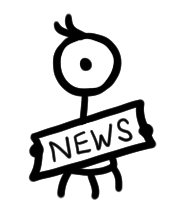
\includegraphics[width=\linewidth]{images/trip/trip11.png}
\end{minipage}

\section{The Commodore 64}
The Commodore 64 uses a MOS technologies 8-bit 6510 microprocessor (a variant of the 6502) clocked in at 0.985 MHz (PAL version). It has a 16 bit address register allowing for $2^16 = 65535 = \$FFFF = 64kb$ of memory, but actually has a bit more than this when ROM (read-only-memory) is included. The "GPU" (graphics chip) of the C64 is called the Video Interface Chip (VIC), and shares the same RAM/ROM as the C64. This means that the data feeding the signal that the VIC chip is producing is directly accessible by the CPU.

When the computer starts up, the VIC screen points to memory address \$0400. When you run a TRSE program, the default memory location for the program is at \$800, but the BASIC is overloaded and told to execute your program (starting at \$810) instead. Let's create a TRSE program that changes a byte on the screen:
\subsection{My First Program}
\begin{lstlisting}
program MostBasicProgram;
begin
	poke(^$0400,0,1);
	Loop();
end.
\end{lstlisting}

\begin{minipage}{0.2\textwidth}
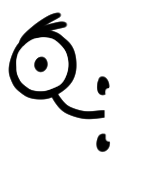
\includegraphics[width=\linewidth]{images/trip/trip12.png}
\end{minipage}
\begin{minipage}{0.8\textwidth}
"Poke" means "Set byte at memory address". Poke(\^\$0400,0,1) therefore translates to "Set the value of memory address \$0400+0 to be "1". Then loop the program ad infinitum. Incidentally, \$0400 is the beginning of screen space, and therefore represents the character in the upper-left corner of the screen. Value "1" corresponds to the ROM screen character for "A".
\end{minipage}

\begin{minipage}{0.8\textwidth}
The VIC addressing is somewhat skewed, since it can only access 16kb of ram. This means that the VIC address space is evenly divided into 4 "banks" on the c64: from \$0000-\$3FFF, \$4000-\$7FFF, \$8000-\$BFFF and finally \$C000-\$FFFF. When you tell the VIC chip to "use bank 2", what you are doing is telling it to access and use memory from \$8000-\$BFFF.
\end{minipage}
\begin{minipage}{0.2\textwidth}
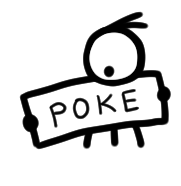
\includegraphics[width=\linewidth]{images/trip/trip7.png}
\end{minipage}


\section{TRSE Tutorials}
\subsection{Hello World}
\begin{minipage}{0.8\textwidth}
\begin{lstlisting}
program HelloWorld;
var  
  	text : string = ("HELLO WORLD");

begin
	// Fill the screen (at screen_char_loc) with character $20 - "space"
	ClearScreen($20, screen_char_loc);
	// Fill the color ram with yellow
	ClearScreen(yellow, screen_col_loc);
	// Move cursor to x,y position 10,12
	moveto(10,12,$04);
	// Print the text
	printstring(text,0,40);
	// Move cursor 2 rows down (2*40)
	screenmemory:=screenmemory+2*40;
	// Print something else
	printstring("THIS IS ANOTHER STRING",0,40);
	// Infinite loop
	Loop(); 
end.
\end{lstlisting}
\end{minipage}
\begin{minipage}{0.2\textwidth}
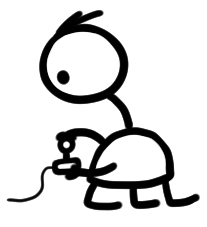
\includegraphics[width=\linewidth]{images/trip/trip8.png}
\end{minipage}

\begin{minipage}{0.6\textwidth}
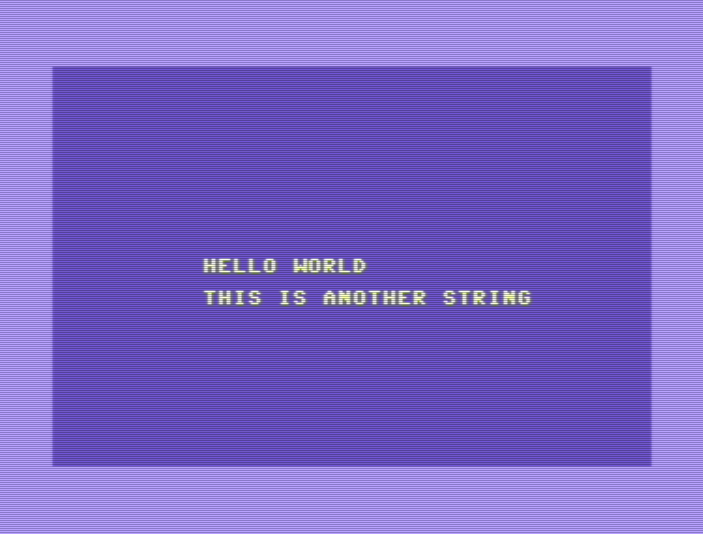
\includegraphics{images/c64/01_helloworld.png}
\end{minipage}
\begin{minipage}{0.4\textwidth}
Lorem ipsum dolor sit amet, quo ex molestiae philosophia. Qui periculis sententiae comprehensam eu, audiam accusamus consequat eum no, no nam legimus placerat. Qui no dictas accusamus, no vim liberavisse instructior. Ius quaeque utroque tincidunt ei, his saperet consequat eu.
\end{minipage}
Te autem impetus ius, vel facer omnes mediocrem in. Timeam persius eligendi at sed, eu vitae noster latine vel. Liberavisse definitiones comprehensam te sea. Pri ne mollis expetenda, cum habeo quaestio maiestatis an. Ne vim senserit sapientem dissentiet. Et vis ceteros lucilius, ad aperiri argumentum vis.


\subsection{Texty}
\begin{minipage}{0.8\textwidth}
\begin{lstlisting}
program Texty;
var  
	// Define three variables : position x, position y and time
   x,y,time,i: byte = 0;  
begin
 	// First, fill color ram with white
	ClearScreen(white, screen_col_loc);
	// Set black border
	screen_bg_col:=black;
	// infinite loop
	while (true) do
	begin
		// Make sure we wait for 1 raster cycle to complete
		waitforraster(0);
		// Clear screen with character $20 (space)
		ClearScreen($20, screen_char_loc);
		// Calculate x,y some sine values (making a circle)
		// if sine[x] then sine[x+64] is equal to cosine  
		x:=sine[time]/12 + 6;		
		y:=sine[time+64]/16 + 4;		
		// move "screenmemory" cursor to x,y at screen memory $0400
		moveto(x,y,$04);
		
		i:=time/64; // i will now have values between 0 and 3 (since time is between 0 and 255)
		// Print some random string
		case i of
			0:	printstring("I AM FISH",0,40);
			1:	printstring("ARE YOU FISH",0,40);
			2:	printstring("ME AM CAT",0,40);
			3:	printstring("OM NOM NOM",0,40);
		end;
		// Increase the timer
		time:=time+1;
	end;

end.
\end{lstlisting}
\end{minipage}
\begin{minipage}{0.2\textwidth}
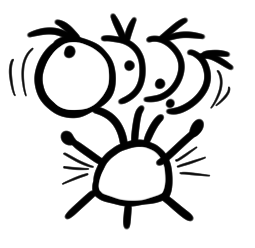
\includegraphics[width=\linewidth]{images/trip/trip9.png}
\end{minipage}

\begin{minipage}{0.4\textwidth}
Lorem ipsum dolor sit amet, quo ex molestiae philosophia. Qui periculis sententiae comprehensam eu, audiam accusamus consequat eum no, no nam legimus placerat. Qui no dictas accusamus, no vim liberavisse instructior. Ius quaeque utroque tincidunt ei, his saperet consequat eu.
\end{minipage}
\begin{minipage}{0.6\textwidth}
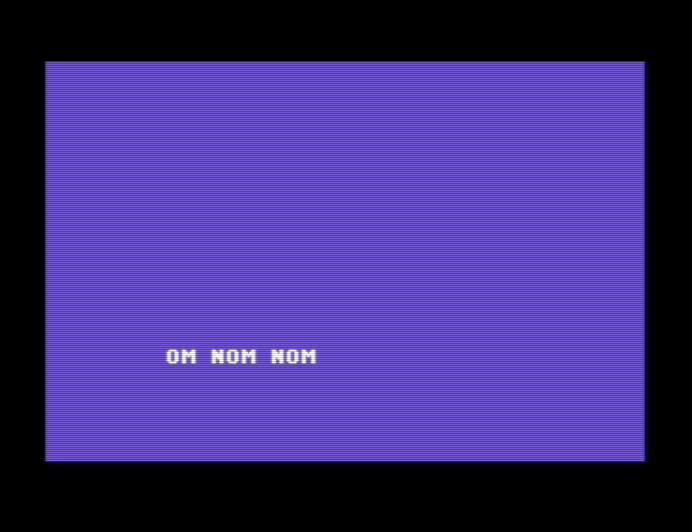
\includegraphics{images/c64/02_texty.png}
\end{minipage}
Te autem impetus ius, vel facer omnes mediocrem in. Timeam persius eligendi at sed, eu vitae noster latine vel. Liberavisse definitiones comprehensam te sea. Pri ne mollis expetenda, cum habeo quaestio maiestatis an. Ne vim senserit sapientem dissentiet. Et vis ceteros lucilius, ad aperiri argumentum vis.


\subsection{Boxes}
\begin{minipage}{0.8\textwidth}
\begin{lstlisting}
program Boxes;
var  
	saddr: array[25] of integer; // Screen address table
	caddr: array[25] of integer; // Color adress table
	
	box: array[8] of byte = ($55, $43, $49, $5d, $4b, $43, $4a, $5d);
	x,y,dx,dy,t: byte = 0;

	
begin
	// Set screen background/border color
	screen_bg_col:=black;
	screen_fg_col:=black;
	
    clearscreen($20, screen_char_loc);
    clearscreen(black, screen_col_loc);
	// Sets up the address tables for the screen & color memory    
	createaddresstable(saddr,screen_char_loc,40,25);
	createaddresstable(caddr,screen_col_loc,40,25);

	// dx and dy are initialized to 1
	dx:=1;
	dy:=1;
	while (true) do begin
		// Make sure we only draw 1 box per frame
		waitforraster(80);
		// Add the delta dx and dy to x and y
		x:=x+dx;
		y:=y+dy;
		// Flip dx and dy when borders are reached
	    case x of
		    	31: dx := -1;
		    	0: dx := 1;
		end;
	    case y of
	    		20: dy := -1;
	    		0: dy := 1;
		end;
		// Make sure that t loops from 0-15
		t:=(t+1)&15;
		// Draw two boxes in opposing corners
		drawcolortextbox(saddr, caddr, box, x, y, 9, 5, t);
		drawcolortextbox(saddr, caddr, box, 31 - x, 20 - y, 9, 5, 16 - t);
	end;
end.\end{lstlisting}
\end{minipage}
\begin{minipage}{0.2\textwidth}
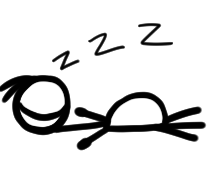
\includegraphics[width=\linewidth]{images/trip/trip10.png}
\end{minipage}

\begin{minipage}{0.4\textwidth}
Lorem ipsum dolor sit amet, quo ex molestiae philosophia. Qui periculis sententiae comprehensam eu, audiam accusamus consequat eum no, no nam legimus placerat. Qui no dictas accusamus, no vim liberavisse instructior. Ius quaeque utroque tincidunt ei, his saperet consequat eu.
\end{minipage}
\begin{minipage}{0.6\textwidth}
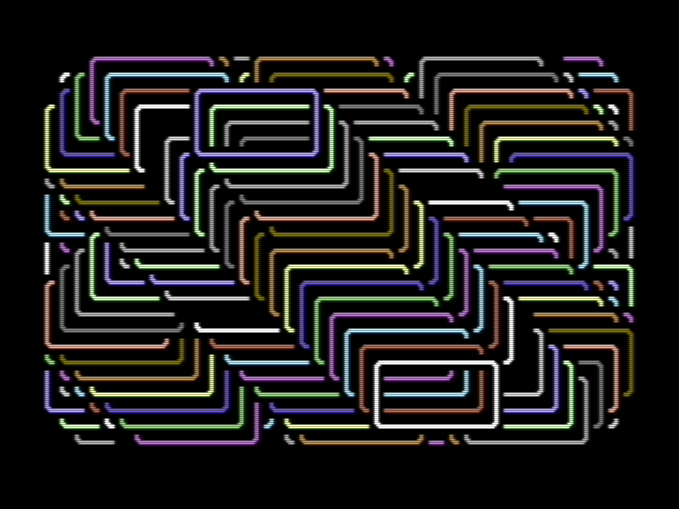
\includegraphics{images/c64/03_boxes.png}
\end{minipage}
Te autem impetus ius, vel facer omnes mediocrem in. Timeam persius eligendi at sed, eu vitae noster latine vel. Liberavisse definitiones comprehensam te sea. Pri ne mollis expetenda, cum habeo quaestio maiestatis an. Ne vim senserit sapientem dissentiet. Et vis ceteros lucilius, ad aperiri argumentum vis.


\subsection{Randomness ahoy!}
\begin{lstlisting}
program Randomness;
var  
	random_color,x,y,index: byte; 
	// Array of random bytes
	random_values : array[256] of byte; 
	// Pointer to screen and color ram
	screenP, colorP : pointer;



// Initialize a random table of 256 bytes
// generator
procedure InitializeRandom();
begin
	// same as : for x:=0 to 0 do begin..
	for x:=0 to 256 do begin 
		random_values[x]:=Random();
    end;
end;

begin
	InitializeRandom();
	// Set screen foreground and background to black. The second parameter is an offset.
	screen_bg_col:=black;
	screen_fg_col:=black;
	
	// point to start of random table
	index:=0; 
	// infinite loop
	while (true) do  begin
		// Set pointer to point to beginning of screen/color ram ($0400 and $D800)
		screenP:=screen_char_loc;
		colorP:=screen_col_loc;
		// loop y		
		for y:=0 to 24 do begin
			// moves current screen position
			// Select some random color
			for x:=0 to 40 do begin
				// Sets both screen and color values
				screenP[x] := random_values[index];
				// increases screen X counter
				// Increase by some random non-repeatable prime
				index:=index+17;
	    		end;
			// Select some random color
			random_color := random_values[index];
			// Fill the current line in colorP with 40 bytes of random_color
			fill(colorP,random_color,40);
			// Increase screen and color pointers
			screenP:=screenP+40;
			colorP:=colorP+40;
			end
	end;

end.
\end{lstlisting}

\begin{minipage}{0.4\textwidth}
Lorem ipsum dolor sit amet, quo ex molestiae philosophia. Qui periculis sententiae comprehensam eu, audiam accusamus consequat eum no, no nam legimus placerat. Qui no dictas accusamus, no vim liberavisse instructior. Ius quaeque utroque tincidunt ei, his saperet consequat eu.
\end{minipage}
\begin{minipage}{0.6\textwidth}
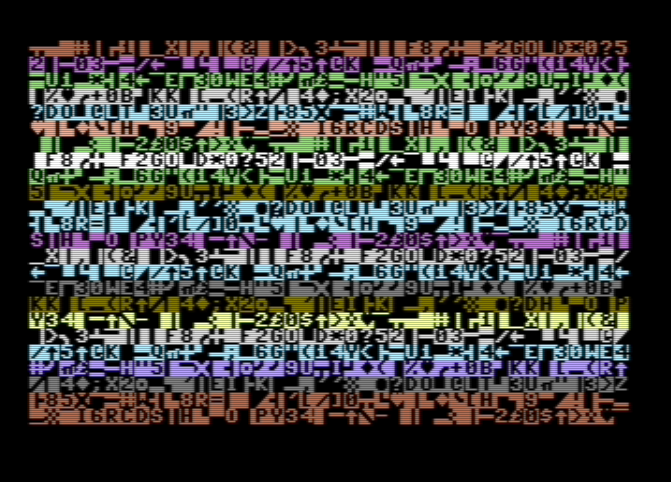
\includegraphics{images/c64/04_randomness.png}
\end{minipage}
Te autem impetus ius, vel facer omnes mediocrem in. Timeam persius eligendi at sed, eu vitae noster latine vel. Liberavisse definitiones comprehensam te sea. Pri ne mollis expetenda, cum habeo quaestio maiestatis an. Ne vim senserit sapientem dissentiet. Et vis ceteros lucilius, ad aperiri argumentum vis.


\subsection{Plasma}
Definitions and arrays.
\\
\begin{minipage}{0.8\textwidth}
\begin{lstlisting}
program Tutorial3_plasma;

var
	// some plasma variables
	c,val,c2x, c2y,ax, ay : byte;
	x,y : byte;
	colorP: pointer;	

// charset will be placed at $2000 in bank 1	
@define charsetLocation $2000
 // look in the character set
@define baseCharacter $68

	// Use custom charset
	charset: IncBin("charsets/charset.bin",@charsetLocation);
	// nice colors
	fade : array [] of byte = (11,6,12,12,4,14,15,1,1,1,1,15,14,4,12,12,6,11,1,1); 
	

	// mini sine table
    siny : array[25] of byte; 
	sinx : array[40] of byte; 

	// Lookup table for division by 16
	lookupDiv16 : array[256] of byte;


// Define y_start as a global preprocessor constant
@define y_start "5"
\end{lstlisting}
\end{minipage}
\begin{minipage}{0.2\textwidth}
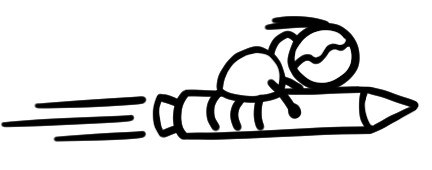
\includegraphics[width=\linewidth]{images/trip/trip13.png}
\end{minipage}

The plasma method itself!\\

\begin{minipage}{0.8\textwidth}
\begin{lstlisting}
procedure Plasma();
begin
	c2x:=ax;
	c2y:=ay;
	
	// Set up y-sine table
	for x:=0 to 25 do begin 
		siny[x]:=  sine[c2x] + sine[c2y];
		c2x:=c2x+4;
		c2y:=c2y+9;
	end;

	ax:=ax+3;
	ay:=ay-5;

	// Set up x-sine table
	for x:=0 to 40 do begin 
		sinx[x] := sine[c2x] + sine[c2y];
		c2x:=c2x+3;
		c2y:=c2y+7;

	end;
	// Move cursor to (1,y) on $0400 on bank 1
	moveto(1,@y_start, $04);
	// moveto could also be replaced with : screenmemory:=$0400 + @y_start*40;
	
	colorP:=screen_col_loc + @y_start*40;
	
	for y:=@y_start to 23 do begin
		val:=siny[y];
		for x:=1 to 36 do begin
			// here, we take (sin[x]+val) and divide by 16. However, since this is a slow procedure,
			// we have created a lookup table instead!
			c:=lookupDiv16[ (sinx[x] +val) ];
			// Set the screen memory
			screenmemory[x]:=c + @baseCharacter;
			// Set color memory
			colorP[x] := fade[ c ];

		end;
		// Increase screen memory pointer by 40 (next row)
		screenmemory:=screenmemory+40;
		// Increase color pointer by 40 (next row)
		colorP:=colorP+40;
	end;

end;
\end{lstlisting}
\end{minipage}

\begin{minipage}{0.2\textwidth}
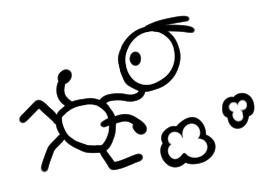
\includegraphics[width=\linewidth]{images/trip/trip14.png}
\end{minipage}


The main method\\
\begin{minipage}{0.8\textwidth}
\begin{lstlisting}
procedure InitDivision16();
begin
	for x:=0 to 256 do lookupDiv16[x]:=x/16; // Simply store values divided by 16
end;

begin
	// Set color background
	screen_bg_col:=black;
	screen_fg_col:=black;
	// Set charmap location at $2000
	SetCharsetLocation(@charsetLocation);
	InitDivision16();
	ax:=1;
	ay:=5;

	// Clear screen and color memory
	ClearScreen($20, screen_char_loc);
	// Main loop
	while (true) do begin
		waitForRaster(0);
		Plasma();
	end;
end.
\end{lstlisting}
\end{minipage}
\begin{minipage}{0.2\textwidth}
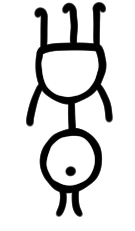
\includegraphics[width=\linewidth]{images/trip/trip15.png}
\end{minipage}




\begin{minipage}{0.6\textwidth}
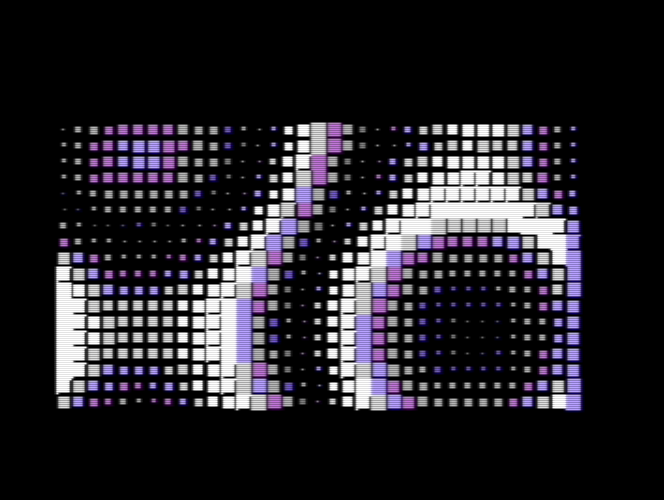
\includegraphics{images/c64/06_plasma.png}
\end{minipage}
\begin{minipage}{0.4\textwidth}
Lorem ipsum dolor sit amet, quo ex molestiae philosophia. Qui periculis sententiae comprehensam eu, audiam accusamus consequat eum no, no nam legimus placerat. Qui no dictas accusamus, no vim liberavisse instructior. Ius quaeque utroque tincidunt ei, his saperet consequat eu.
\end{minipage}
Te autem impetus ius, vel facer omnes mediocrem in. Timeam persius eligendi at sed, eu vitae noster latine vel. Liberavisse definitiones comprehensam te sea. Pri ne mollis expetenda, cum habeo quaestio maiestatis an. Ne vim senserit sapientem dissentiet. Et vis ceteros lucilius, ad aperiri argumentum vis.


\section{What's an interrupt?}
Imagine you are painting your apartement - in the 20th floor. Since you have to be finished by tomorrow, you have asked three of your friends to come help you. But the problem is that you don't know exactly when each of them will show up. 
\\
Now, why is it a problem that you don't know exactly when they show up you may wonder? The door bell on the 1st floor is broken. So you constantly have to run down from the 20th floor, open the door, check for friends, run back up, paint 30 seconds, run down again to the 1st floor, open the door, check for friends, run back up, paint 30 seconds, run do..... ok! You get the point. The only thing you will be busy with is waiting. Ideally, you would like to start painting your apartement and just be INTERRUPTED when each of your friends ring the door bell. But since this interrupt mechanism is broken, you need to find another solution: the mobile phone.
\\
So, instead you call your friends and tell them to use their mobile phones to ring you when they are downstairs. In that way you can constantly keep painting, and be notified (INTERRUPTED) only when you friends are ready downstairs.
\\
What's this story do to with programming the C64 with TRSE? Well, of course this was just an analogy. But if we want to make smart and effective programs we need to have the 6510 CPU work at full speed - with real tasks - and only be interrupted when something important happens! And when the interrupt routine is completed the CPU goes back to the tasks it was interrupted from.
\\
Ok, let's gets started! 
\\
\subsection{Avoiding busy waits - our first simple interrupt routine}
In the story above you see that it is possible to constantly run up and down to check for you friends, but it's not very effective. The same goes for the C64 - you can have the CPU to just sit and wait for something to happen (BUSY WAIT).  

Let's look at an example. Below you find a small program that set the background color to black at line 0, and turn it to yellow at line 150. Copy and paste this sample into TRSE and run it!
\begin{lstlisting}
program BusyWait;
var

procedure MainLoop();
begin
	WaitForRaster(0);
	SCREEN_BG_COL:=BLACK;
	
	WaitForRaster(150);
	SCREEN_BG_COL:=YELLOW;
end;

begin
	while(0<1) then begin
		MainLoop();
	end;
end.
\end{lstlisting}What is the problem with this program? It's switching from black to yellow? Well, the function WaitForRaster() prevents the CPU of doing anything else while waiting. In a real program you would like to do a lot of stuff while waiting for a rasterline such as calculating new sprite positions, moving a scrolltext, preparing a new screen in a different videobank etc. 

Now, how would this program look if we would like to use interrupts instead? It would look like this: 
\begin{lstlisting}
program RasterInterrupt;
var  
	@define useKernal 0
	
interrupt InterruptRoutine02();

interrupt InterruptRoutine01();
begin
	StartIRQ(@useKernal);
	SCREEN_BG_COL:=BLACK;

	RasterIRQ(InterruptRoutine02(),150,@useKernal);
	
	CloseIRQ();
end;

interrupt InterruptRoutine02();
begin
	StartIRQ(@useKernal);
	SCREEN_BG_COL:=YELLOW;

	RasterIRQ(InterruptRoutine01(),0,@useKernal);
	
	CloseIRQ();
end;

procedure MainLoop();
begin
	// Insert your program here
end;


begin
	preventirq();
	disableciainterrupts();
	setmemoryconfig(1,@useKernal,0);
	enablerasterirq();
	rasterirq(InterruptRoutine01(),0,@useKernal);
	enableirq();

	while (0<1) then begin
		MainLoop();
	end;
end.
\end{lstlisting}
First of all note this: the MainLoop() does NOTHING now! This means that you are now free to do anything you like in the MainLoop, and the background will still be colored black and yellow! The interrupts does this for you! 

Lets's go trough the program and explain everything step-by-step!








busy waits
different types of interrupts
needs to be masked






broken = masked

Types of interrupts on the C64 (NMI, BRK, CIA, VICs)

KERNAL vs HW

Basics of interrupts

	- Trigger
	- Interrupt routine
	- Acknowledge
	- Return

Sample - VIC raster interrupt


